\section{Improving Analysis using Multi-Context Information}
\label{sec:context}
In this section we describe our design goals of usage of each context.
We describe how we extract the context from multiple data sources.
Also, we show how the context is visually incorporated into the system.

\subsection{Keyword Extraction and Visualization}
%Trajectory clusters indicate common movements. 
%Those who move similarly and stay in the neighborhood at the same time period may experience common situations.
Analyzing the spatial behaviors alone is limited in achieving situational awareness of local events\textemdash they cannot answer why people move and what situations occur.
To address this  challenge, we extract keywords from the tweets used to generate a trajectory cluster and also those located close to the cluster, because such Tweets can contain common topics indicating an event occurring around a similar mobility.
Then we display the extracted keywords for providing additional insights into the event and the mobility patterns.

%\textbf{Keyword extraction:}
We select a set of Tweets that constitute sub-trajectories belonging to a cluster and are located within a specific distance to the representative trajectory of the cluster.
In this work, the default value of the distance threshold is set to 200 meters.
Then, we extract keywords from the text of the selected Tweets.
We calculate the frequencies of each word in the aggregate text and select top keywords based on the frequencies.
%The number of selected keywords depends on the number of selected tweets (maximum: 15 and minimum: 2).

%\textbf{Keyword visualization:} 
To display the extracted keywords, we utilize \textquoteleft tag cloud\textquoteright visualization.
Tag clouds have been used to represent a most frequent or important words in order to summarize text collections~\cite{Viegas:2008:Timelines}.
Also, tag clouds can be exploited for analytics tasks, such as topic-based document navigation and labeling geographical points of interest~\cite{Thom:2012:SAD,Luboschik:2008:Particle}.
In this work, we display the keywords along their corresponding representative trajectory without overlapping.
%Once the users hover a mouse pointer over a representative trajectory, it becomes darker and its keywords appear to avoid visual clutter.
The font size of each keyword encodes the frequency to show the popularity of the keyword.
Figure~\ref{fig:keyword_photo} (top) shows an example of showing extracted keywords display along the center trajectory. 
%The details on data will be explained in Section~\ref{sec:boston_marathon}.
%In case of overlapping trajectories, the shorter or thinner one under the mouse pointer will be selected. 
%The users can browse over the distributed trajectories to see if they have important keywords.

%~\cite{Nabo:2014:Annotating}
%In this work, we use tweets with geo-location, one of popular microblog services, which provide textual information, and geo-tagged photographs from photo sharing social network services (i.e., Instagram) and geo-tagged Tweets containing photographs provide image information.
\begin{figure}[htb]
	\centering
	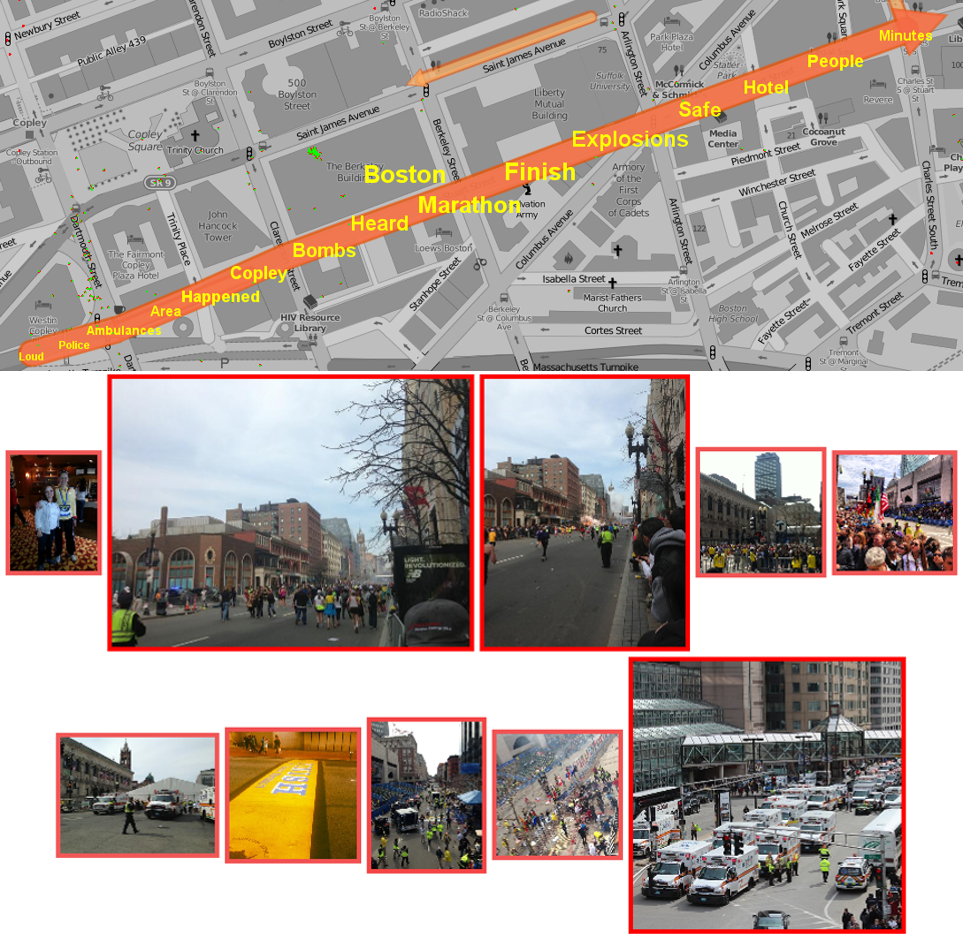
\includegraphics[width=1.0\linewidth]{keyword_photo_v2}
	\caption{
The extracted keywords along the trajectory close to the explosion locations show a strong relationship to the explosions (top).
The chronologically displayed photos (bottom) extracted from the same trajectory show the scenes of evolving situations.
}
	\label{fig:keyword_photo}
	%\vspace{-0.4cm}
\end{figure}

%\subsection{Improving situational awareness by shared photo, live public cameras, and news media}
\subsection{Additional Context Information}
For additional context, we utilize shared photos, public web camera videos, and news media related to each representative trajectory.
These data sources provide additional channels of information to users; thereby, providing a more comprehensive situational awareness for any emerging situation. 
%This context provide additional channels of information.
%Therefore, visualizations of the context can provide a more comprehensive view and improve movement analysis

\textbf{Shared photos:}
Right after people take photos, they can post the photos to LBSNs with their smartphones.
%A huge number of tweets include photos.
For example, we collected more than 230 of Tweets with photos were generated within the first 5 hours after the explosions at the Boston Marathon in 2013.
%1129 tweets with photos were generated during about 24 hours after the explosions at the Boston Marathon. 
The photos allow first responders and emergency managers to obtain a better situational awareness of what is happening on the site during a crisis.

In our system, we first select the Tweets in the same manner as for keyword extraction.
we identify Tweets with photos from the selected tweets for each trajectory cluster; tweets with photos contain photo links in a particular format.
Images are retrieved from links within Tweets and displayed chronologically in a separate window (e.g., as shown in Figure~\ref{fig:keyword_photo}).
%Then we extract the photo links and retrieve photos.
%These photos are chronologically displayed in a separate window to provide their temporal attributes.
Photo sizes correspond to relative differences in their sharing count (sum of retweets and replies)~\cite{Dork:2010:Visual}.
When a photo is selected, the location of the photo's Tweet is highlighted on the map.

\textbf{Public live web camera videos:}
%Even though there are quite a few public live web camera videos available online, use of implicit streaming data have a strong possibility to improve the temporal understanding of the situation at the site~\cite{Bergstrand:2011:VRT}.
We utilize public webcam video feeds to allow the emergency managers to obtain a better situational awareness of an emerging crises situation~\cite{Bergstrand:2011:VRT}.
In our system, we mark available camera locations on the map with pre-loaded camera location data~\cite{Purdue:2014:Webcam}.
Once users click on one of the web cameras icons on the map, the live streaming feed or most recent snapshots are provided (e.g., as shown in Figure~\ref{fig:purdue_shooting}).

\textbf{News media:}
%Sometimes information in social media provided by the public can be insufficient and inaccurate.
%However, news media reports from major news agencies are generally more abundant and accurate than one from the public.
We augment the information provided by the public in social media with news media reports from major news agencies.
News media reports related to the context of movements can provide more reliable information.
We search news reports with extracted keywords from nearby Tweets for each cluster using the Google search APIs.
The results, including titles, summaries and links of each news report, are displayed in a separate window.

\begin{figure}[htb]
	\centering
	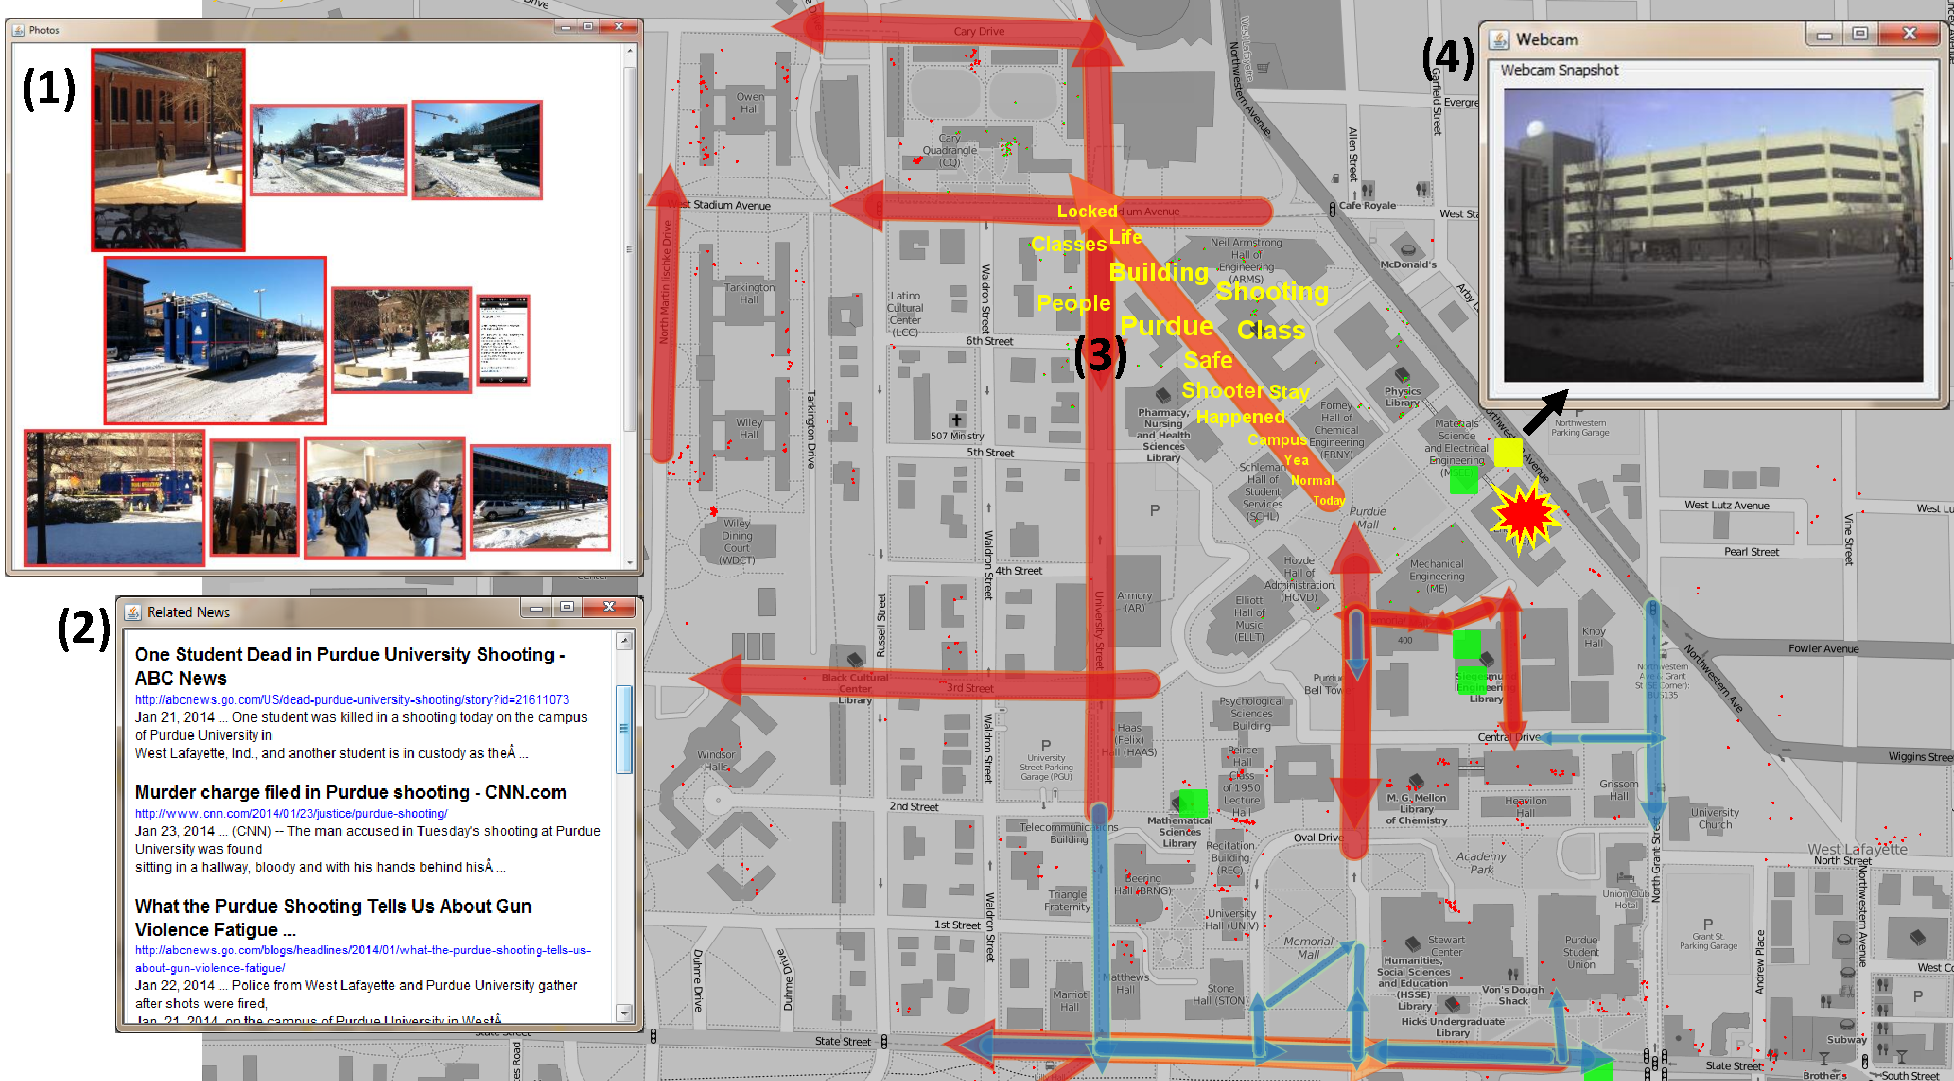
\includegraphics[width=1.0\linewidth]{purdue_shooting_v2}
	\caption{	
	The trajectories (red and orange) shows the human movements around the campus during 2 hours after the shooting.
	The normal trajectories (blue) extracted from the same time period on normal day.
	Photos (1), News reports (2), Keywords (3), and Webcam videos (4).
	The green rectangles indicate the locations of the web cameras around the campus. The yellow one is the selected camera.
	The marker indicate the building where the accident occurred.
	}
	\label{fig:purdue_shooting}
	%\vspace{-0.4cm}
\end{figure}